\begin{frame}{Zugfolge f�r $n=4$ und $k=5$}
\only<0>{
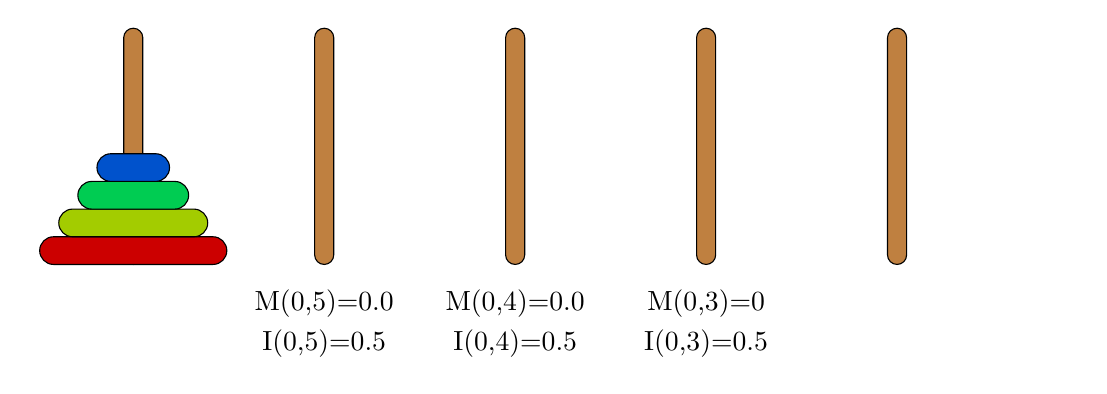
\begin{tikzpicture}
\pgfmathsetlengthmacro\diskheight{10};
\pgfmathsetmacro\k{5};
\pgfmathsetlengthmacro\step{\textwidth/\k};
\draw[color = white] (\step/2,0) -- (\textwidth+\step,0);
\foreach \n in {1,...,\k} \draw [fill = brown, draw = black, rounded corners = \step/20] (\step*\n,0) rectangle (\step*\n+\step/10,3);
\node (2) at (\step*2.05,-0.5){M(0,5)=0.0};
\node (2) at (\step*2.05,-1){I(0,5)=0.5};
\node (3) at (\step*3.05,-0.5){M(0,4)=0.0};
\node (3) at (\step*3.05,-1){I(0,4)=0.5};
\node (4) at (\step*4.05,-0.5){M(0,3)=0};
\node (4) at (\step*4.05,-1){I(0,3)=0.5};
\definecolor{mycolor}{rgb:hsb}{0.00,1,0.8}
\draw [fill = mycolor, draw = black, rounded corners = \diskheight/2] (\step*1+\step/20-\step*0.49,\diskheight*0) rectangle (\step*1+\step/20+\step*0.49,\diskheight*1);
\definecolor{mycolor}{rgb:hsb}{0.20,1,0.8}
\draw [fill = mycolor, draw = black, rounded corners = \diskheight/2] (\step*1+\step/20-\step*0.39,\diskheight*1) rectangle (\step*1+\step/20+\step*0.39,\diskheight*2);
\definecolor{mycolor}{rgb:hsb}{0.40,1,0.8}
\draw [fill = mycolor, draw = black, rounded corners = \diskheight/2] (\step*1+\step/20-\step*0.29,\diskheight*2) rectangle (\step*1+\step/20+\step*0.29,\diskheight*3);
\definecolor{mycolor}{rgb:hsb}{0.60,1,0.8}
\draw [fill = mycolor, draw = black, rounded corners = \diskheight/2] (\step*1+\step/20-\step*0.18999999999999995,\diskheight*3) rectangle (\step*1+\step/20+\step*0.18999999999999995,\diskheight*4);
\end{tikzpicture}
}
\only<1>{
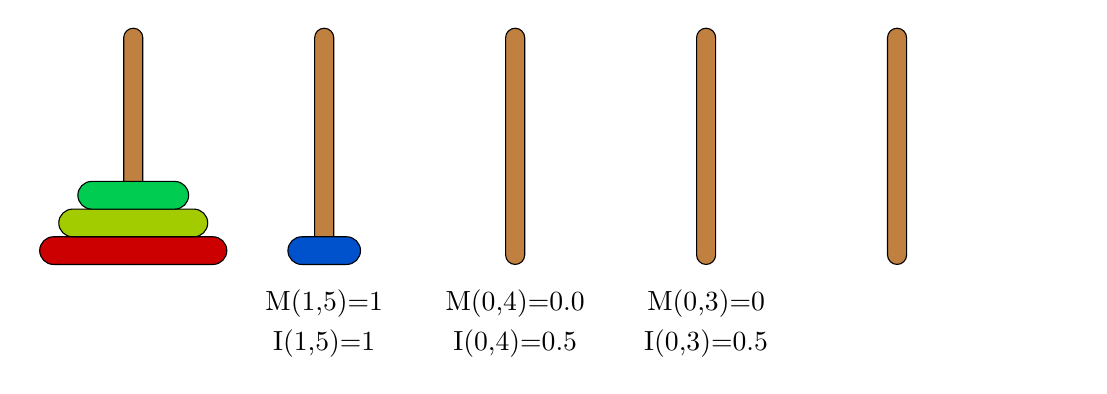
\begin{tikzpicture}
\pgfmathsetlengthmacro\diskheight{10};
\pgfmathsetmacro\k{5};
\pgfmathsetlengthmacro\step{\textwidth/\k};
\draw[color = white] (\step/2,0) -- (\textwidth+\step,0);
\foreach \n in {1,...,\k} \draw [fill = brown, draw = black, rounded corners = \step/20] (\step*\n,0) rectangle (\step*\n+\step/10,3);
\node (2) at (\step*2.05,-0.5){M(1,5)=1};
\node (2) at (\step*2.05,-1){I(1,5)=1};
\node (3) at (\step*3.05,-0.5){M(0,4)=0.0};
\node (3) at (\step*3.05,-1){I(0,4)=0.5};
\node (4) at (\step*4.05,-0.5){M(0,3)=0};
\node (4) at (\step*4.05,-1){I(0,3)=0.5};
\definecolor{mycolor}{rgb:hsb}{0.00,1,0.8}
\draw [fill = mycolor, draw = black, rounded corners = \diskheight/2] (\step*1+\step/20-\step*0.49,\diskheight*0) rectangle (\step*1+\step/20+\step*0.49,\diskheight*1);
\definecolor{mycolor}{rgb:hsb}{0.20,1,0.8}
\draw [fill = mycolor, draw = black, rounded corners = \diskheight/2] (\step*1+\step/20-\step*0.39,\diskheight*1) rectangle (\step*1+\step/20+\step*0.39,\diskheight*2);
\definecolor{mycolor}{rgb:hsb}{0.40,1,0.8}
\draw [fill = mycolor, draw = black, rounded corners = \diskheight/2] (\step*1+\step/20-\step*0.29,\diskheight*2) rectangle (\step*1+\step/20+\step*0.29,\diskheight*3);
\definecolor{mycolor}{rgb:hsb}{0.60,1,0.8}
\draw [fill = mycolor, draw = black, rounded corners = \diskheight/2] (\step*2+\step/20-\step*0.18999999999999995,\diskheight*0) rectangle (\step*2+\step/20+\step*0.18999999999999995,\diskheight*1);
\end{tikzpicture}
}
\only<2>{
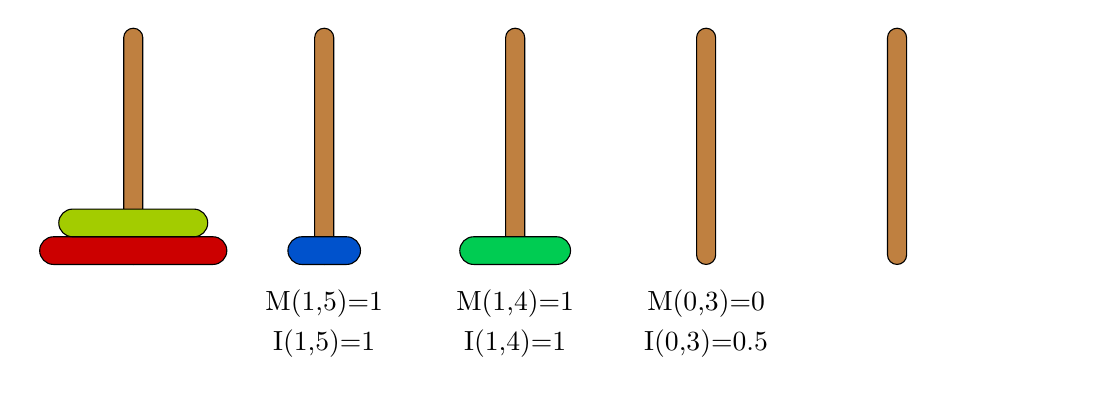
\begin{tikzpicture}
\pgfmathsetlengthmacro\diskheight{10};
\pgfmathsetmacro\k{5};
\pgfmathsetlengthmacro\step{\textwidth/\k};
\draw[color = white] (\step/2,0) -- (\textwidth+\step,0);
\foreach \n in {1,...,\k} \draw [fill = brown, draw = black, rounded corners = \step/20] (\step*\n,0) rectangle (\step*\n+\step/10,3);
\node (2) at (\step*2.05,-0.5){M(1,5)=1};
\node (2) at (\step*2.05,-1){I(1,5)=1};
\node (3) at (\step*3.05,-0.5){M(1,4)=1};
\node (3) at (\step*3.05,-1){I(1,4)=1};
\node (4) at (\step*4.05,-0.5){M(0,3)=0};
\node (4) at (\step*4.05,-1){I(0,3)=0.5};
\definecolor{mycolor}{rgb:hsb}{0.00,1,0.8}
\draw [fill = mycolor, draw = black, rounded corners = \diskheight/2] (\step*1+\step/20-\step*0.49,\diskheight*0) rectangle (\step*1+\step/20+\step*0.49,\diskheight*1);
\definecolor{mycolor}{rgb:hsb}{0.20,1,0.8}
\draw [fill = mycolor, draw = black, rounded corners = \diskheight/2] (\step*1+\step/20-\step*0.39,\diskheight*1) rectangle (\step*1+\step/20+\step*0.39,\diskheight*2);
\definecolor{mycolor}{rgb:hsb}{0.60,1,0.8}
\draw [fill = mycolor, draw = black, rounded corners = \diskheight/2] (\step*2+\step/20-\step*0.18999999999999995,\diskheight*0) rectangle (\step*2+\step/20+\step*0.18999999999999995,\diskheight*1);
\definecolor{mycolor}{rgb:hsb}{0.40,1,0.8}
\draw [fill = mycolor, draw = black, rounded corners = \diskheight/2] (\step*3+\step/20-\step*0.29,\diskheight*0) rectangle (\step*3+\step/20+\step*0.29,\diskheight*1);
\end{tikzpicture}
}
\only<3>{
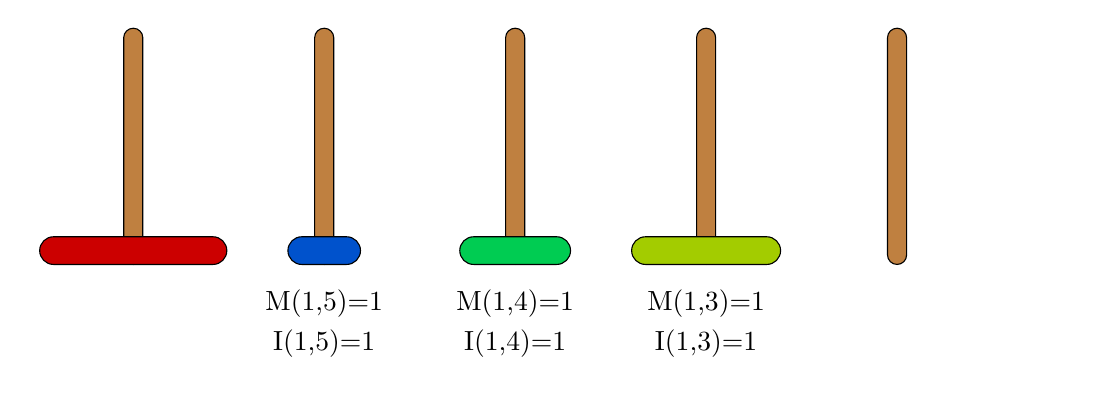
\begin{tikzpicture}
\pgfmathsetlengthmacro\diskheight{10};
\pgfmathsetmacro\k{5};
\pgfmathsetlengthmacro\step{\textwidth/\k};
\draw[color = white] (\step/2,0) -- (\textwidth+\step,0);
\foreach \n in {1,...,\k} \draw [fill = brown, draw = black, rounded corners = \step/20] (\step*\n,0) rectangle (\step*\n+\step/10,3);
\node (2) at (\step*2.05,-0.5){M(1,5)=1};
\node (2) at (\step*2.05,-1){I(1,5)=1};
\node (3) at (\step*3.05,-0.5){M(1,4)=1};
\node (3) at (\step*3.05,-1){I(1,4)=1};
\node (4) at (\step*4.05,-0.5){M(1,3)=1};
\node (4) at (\step*4.05,-1){I(1,3)=1};
\definecolor{mycolor}{rgb:hsb}{0.00,1,0.8}
\draw [fill = mycolor, draw = black, rounded corners = \diskheight/2] (\step*1+\step/20-\step*0.49,\diskheight*0) rectangle (\step*1+\step/20+\step*0.49,\diskheight*1);
\definecolor{mycolor}{rgb:hsb}{0.60,1,0.8}
\draw [fill = mycolor, draw = black, rounded corners = \diskheight/2] (\step*2+\step/20-\step*0.18999999999999995,\diskheight*0) rectangle (\step*2+\step/20+\step*0.18999999999999995,\diskheight*1);
\definecolor{mycolor}{rgb:hsb}{0.40,1,0.8}
\draw [fill = mycolor, draw = black, rounded corners = \diskheight/2] (\step*3+\step/20-\step*0.29,\diskheight*0) rectangle (\step*3+\step/20+\step*0.29,\diskheight*1);
\definecolor{mycolor}{rgb:hsb}{0.20,1,0.8}
\draw [fill = mycolor, draw = black, rounded corners = \diskheight/2] (\step*4+\step/20-\step*0.39,\diskheight*0) rectangle (\step*4+\step/20+\step*0.39,\diskheight*1);
\end{tikzpicture}
}
\only<4>{
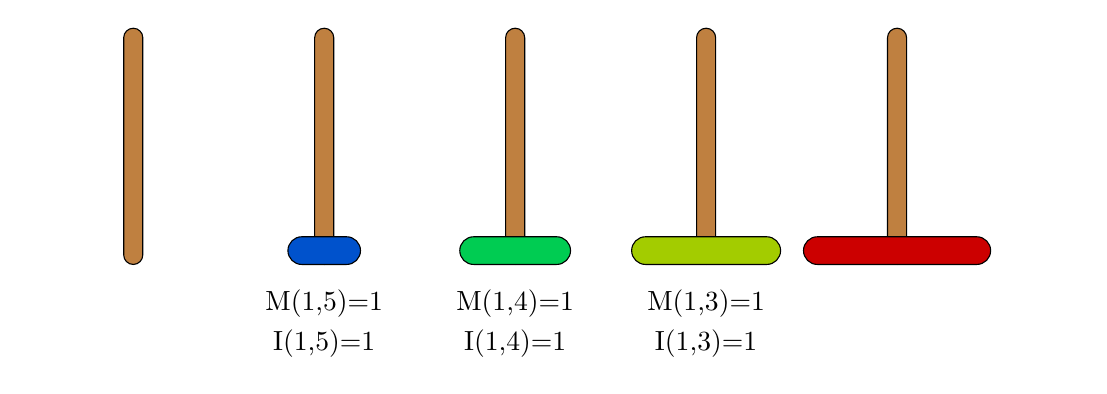
\begin{tikzpicture}
\pgfmathsetlengthmacro\diskheight{10};
\pgfmathsetmacro\k{5};
\pgfmathsetlengthmacro\step{\textwidth/\k};
\draw[color = white] (\step/2,0) -- (\textwidth+\step,0);
\foreach \n in {1,...,\k} \draw [fill = brown, draw = black, rounded corners = \step/20] (\step*\n,0) rectangle (\step*\n+\step/10,3);
\node (2) at (\step*2.05,-0.5){M(1,5)=1};
\node (2) at (\step*2.05,-1){I(1,5)=1};
\node (3) at (\step*3.05,-0.5){M(1,4)=1};
\node (3) at (\step*3.05,-1){I(1,4)=1};
\node (4) at (\step*4.05,-0.5){M(1,3)=1};
\node (4) at (\step*4.05,-1){I(1,3)=1};
\definecolor{mycolor}{rgb:hsb}{0.60,1,0.8}
\draw [fill = mycolor, draw = black, rounded corners = \diskheight/2] (\step*2+\step/20-\step*0.18999999999999995,\diskheight*0) rectangle (\step*2+\step/20+\step*0.18999999999999995,\diskheight*1);
\definecolor{mycolor}{rgb:hsb}{0.40,1,0.8}
\draw [fill = mycolor, draw = black, rounded corners = \diskheight/2] (\step*3+\step/20-\step*0.29,\diskheight*0) rectangle (\step*3+\step/20+\step*0.29,\diskheight*1);
\definecolor{mycolor}{rgb:hsb}{0.20,1,0.8}
\draw [fill = mycolor, draw = black, rounded corners = \diskheight/2] (\step*4+\step/20-\step*0.39,\diskheight*0) rectangle (\step*4+\step/20+\step*0.39,\diskheight*1);
\definecolor{mycolor}{rgb:hsb}{0.00,1,0.8}
\draw [fill = mycolor, draw = black, rounded corners = \diskheight/2] (\step*5+\step/20-\step*0.49,\diskheight*0) rectangle (\step*5+\step/20+\step*0.49,\diskheight*1);
\end{tikzpicture}
}
\only<5>{
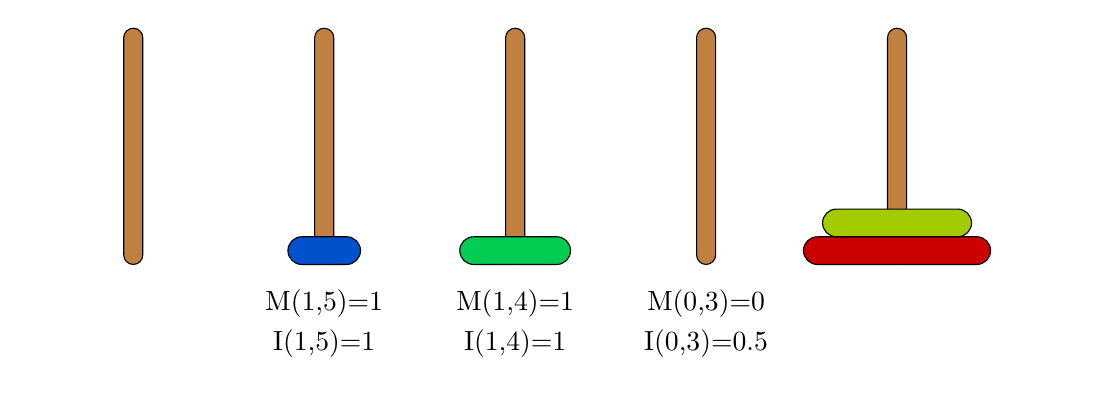
\begin{tikzpicture}
\pgfmathsetlengthmacro\diskheight{10};
\pgfmathsetmacro\k{5};
\pgfmathsetlengthmacro\step{\textwidth/\k};
\draw[color = white] (\step/2,0) -- (\textwidth+\step,0);
\foreach \n in {1,...,\k} \draw [fill = brown, draw = black, rounded corners = \step/20] (\step*\n,0) rectangle (\step*\n+\step/10,3);
\node (2) at (\step*2.05,-0.5){M(1,5)=1};
\node (2) at (\step*2.05,-1){I(1,5)=1};
\node (3) at (\step*3.05,-0.5){M(1,4)=1};
\node (3) at (\step*3.05,-1){I(1,4)=1};
\node (4) at (\step*4.05,-0.5){M(0,3)=0};
\node (4) at (\step*4.05,-1){I(0,3)=0.5};
\definecolor{mycolor}{rgb:hsb}{0.60,1,0.8}
\draw [fill = mycolor, draw = black, rounded corners = \diskheight/2] (\step*2+\step/20-\step*0.18999999999999995,\diskheight*0) rectangle (\step*2+\step/20+\step*0.18999999999999995,\diskheight*1);
\definecolor{mycolor}{rgb:hsb}{0.40,1,0.8}
\draw [fill = mycolor, draw = black, rounded corners = \diskheight/2] (\step*3+\step/20-\step*0.29,\diskheight*0) rectangle (\step*3+\step/20+\step*0.29,\diskheight*1);
\definecolor{mycolor}{rgb:hsb}{0.00,1,0.8}
\draw [fill = mycolor, draw = black, rounded corners = \diskheight/2] (\step*5+\step/20-\step*0.49,\diskheight*0) rectangle (\step*5+\step/20+\step*0.49,\diskheight*1);
\definecolor{mycolor}{rgb:hsb}{0.20,1,0.8}
\draw [fill = mycolor, draw = black, rounded corners = \diskheight/2] (\step*5+\step/20-\step*0.39,\diskheight*1) rectangle (\step*5+\step/20+\step*0.39,\diskheight*2);
\end{tikzpicture}
}
\only<6>{
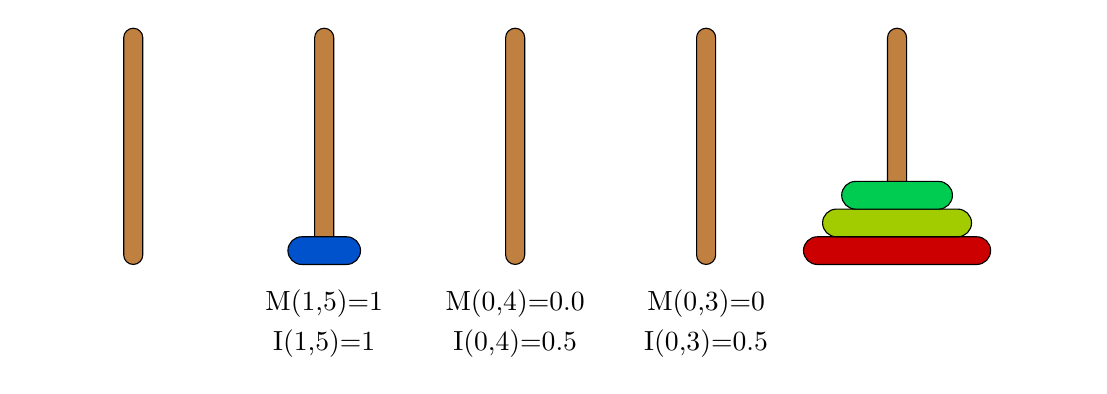
\begin{tikzpicture}
\pgfmathsetlengthmacro\diskheight{10};
\pgfmathsetmacro\k{5};
\pgfmathsetlengthmacro\step{\textwidth/\k};
\draw[color = white] (\step/2,0) -- (\textwidth+\step,0);
\foreach \n in {1,...,\k} \draw [fill = brown, draw = black, rounded corners = \step/20] (\step*\n,0) rectangle (\step*\n+\step/10,3);
\node (2) at (\step*2.05,-0.5){M(1,5)=1};
\node (2) at (\step*2.05,-1){I(1,5)=1};
\node (3) at (\step*3.05,-0.5){M(0,4)=0.0};
\node (3) at (\step*3.05,-1){I(0,4)=0.5};
\node (4) at (\step*4.05,-0.5){M(0,3)=0};
\node (4) at (\step*4.05,-1){I(0,3)=0.5};
\definecolor{mycolor}{rgb:hsb}{0.60,1,0.8}
\draw [fill = mycolor, draw = black, rounded corners = \diskheight/2] (\step*2+\step/20-\step*0.18999999999999995,\diskheight*0) rectangle (\step*2+\step/20+\step*0.18999999999999995,\diskheight*1);
\definecolor{mycolor}{rgb:hsb}{0.00,1,0.8}
\draw [fill = mycolor, draw = black, rounded corners = \diskheight/2] (\step*5+\step/20-\step*0.49,\diskheight*0) rectangle (\step*5+\step/20+\step*0.49,\diskheight*1);
\definecolor{mycolor}{rgb:hsb}{0.20,1,0.8}
\draw [fill = mycolor, draw = black, rounded corners = \diskheight/2] (\step*5+\step/20-\step*0.39,\diskheight*1) rectangle (\step*5+\step/20+\step*0.39,\diskheight*2);
\definecolor{mycolor}{rgb:hsb}{0.40,1,0.8}
\draw [fill = mycolor, draw = black, rounded corners = \diskheight/2] (\step*5+\step/20-\step*0.29,\diskheight*2) rectangle (\step*5+\step/20+\step*0.29,\diskheight*3);
\end{tikzpicture}
}
\only<7>{
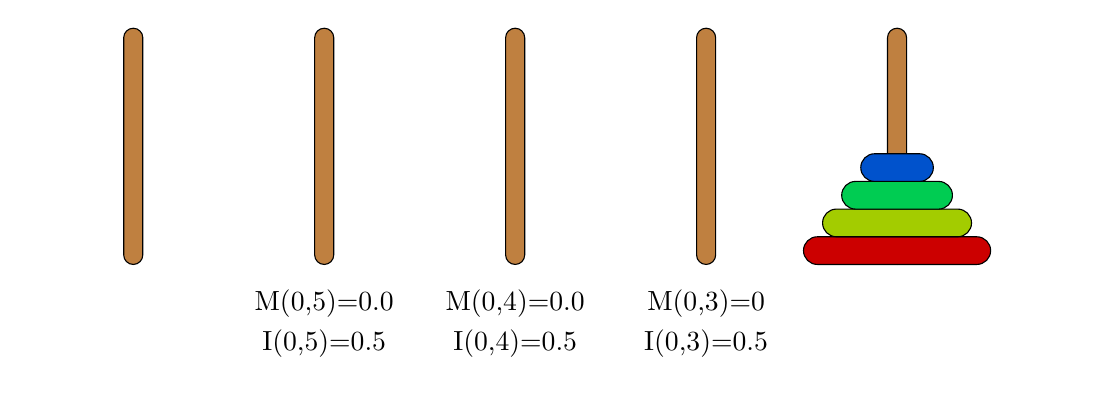
\begin{tikzpicture}
\pgfmathsetlengthmacro\diskheight{10};
\pgfmathsetmacro\k{5};
\pgfmathsetlengthmacro\step{\textwidth/\k};
\draw[color = white] (\step/2,0) -- (\textwidth+\step,0);
\foreach \n in {1,...,\k} \draw [fill = brown, draw = black, rounded corners = \step/20] (\step*\n,0) rectangle (\step*\n+\step/10,3);
\node (2) at (\step*2.05,-0.5){M(0,5)=0.0};
\node (2) at (\step*2.05,-1){I(0,5)=0.5};
\node (3) at (\step*3.05,-0.5){M(0,4)=0.0};
\node (3) at (\step*3.05,-1){I(0,4)=0.5};
\node (4) at (\step*4.05,-0.5){M(0,3)=0};
\node (4) at (\step*4.05,-1){I(0,3)=0.5};
\definecolor{mycolor}{rgb:hsb}{0.00,1,0.8}
\draw [fill = mycolor, draw = black, rounded corners = \diskheight/2] (\step*5+\step/20-\step*0.49,\diskheight*0) rectangle (\step*5+\step/20+\step*0.49,\diskheight*1);
\definecolor{mycolor}{rgb:hsb}{0.20,1,0.8}
\draw [fill = mycolor, draw = black, rounded corners = \diskheight/2] (\step*5+\step/20-\step*0.39,\diskheight*1) rectangle (\step*5+\step/20+\step*0.39,\diskheight*2);
\definecolor{mycolor}{rgb:hsb}{0.40,1,0.8}
\draw [fill = mycolor, draw = black, rounded corners = \diskheight/2] (\step*5+\step/20-\step*0.29,\diskheight*2) rectangle (\step*5+\step/20+\step*0.29,\diskheight*3);
\definecolor{mycolor}{rgb:hsb}{0.60,1,0.8}
\draw [fill = mycolor, draw = black, rounded corners = \diskheight/2] (\step*5+\step/20-\step*0.18999999999999995,\diskheight*3) rectangle (\step*5+\step/20+\step*0.18999999999999995,\diskheight*4);
\end{tikzpicture}
}
\end{frame}